\chapter{System Implementation and Deployment}
\label{chap:implementation}

The preceding chapters describe AI Compass's content pipeline, recommendation logic, retrieval-augmented assistant, and deep-media processing as subsystems. This chapter describes how those subsystems are actually built, hosted, secured, and monetized as a running production system, as of commit \texttt{d6d9421}, the most recent infrastructure change made during this project. The deployment topology described here is the current, live one, confirmed at the commit level rather than inferred from documentation; where the project's own written deployment documentation lags behind the code, that divergence is noted explicitly rather than silently repeated. Two genuine infrastructure pivots occurred during the project's life, each forced by a concrete constraint rather than a change of mind, and both are presented as legitimate engineering narrative rather than something to omit.

\section{Deployment Topology}
\label{sec:impl-topology}

Figure~\ref{fig:deployment} shows the production topology as it currently stands. The frontend is a Next.js~16 / React~19 single-page application, hosted on Vercel, and has remained on Vercel unchanged for the whole project; it owns the entirety of the user interface; every screen a user sees is rendered by this application, with no server-rendered pages served directly by the backend. The backend, comprising the Django application, its Celery workers, and its database, runs on a single AWS EC2 virtual machine. That machine serves the backend over plain HTTP on port 80, with no domain name attached to it, and this is a deliberate rather than accidental choice: the deployment configuration's own comments state directly that Let's Encrypt cannot issue a TLS certificate for a bare IP address, so rather than purchase and maintain a domain name for a small, unfunded student project, the team chose to run the backend over plain HTTP and rely on the frontend being the only HTTPS-facing surface in the whole system. The database is PostgreSQL~16 with the pgvector extension, self-hosted as a container on the same EC2 instance as the Django backend, not exposed on any host port reachable from outside that machine.

The path from a user's browser to this backend is not a direct one. The browser never talks to the EC2 backend at all; instead, Vercel's own Next.js configuration proxies a fixed set of path prefixes (\texttt{/api}, \texttt{/admin}, \texttt{/accounts}, \texttt{/behavior}, \texttt{/assistant}, \texttt{/healthz}, and \texttt{/static}) to the backend server-side, as a server-to-server HTTP hop that the browser itself never sees or participates in. From the browser's point of view, every request, whether it is ultimately served by Vercel's own rendering or forwarded to the Django backend, goes to Vercel's single HTTPS domain. This has a second, load-bearing consequence beyond topology: because the backend is reachable only over plain HTTP, a browser on an HTTPS page attempting to call it directly would be blocked by the browser's own mixed-content policy. Routing every backend-bound request through a server-side proxy on the same origin the page was served from sidesteps that problem entirely, which is precisely why the proxy exists rather than the frontend simply being configured with the backend's raw address.

Tracing a request end to end: a browser request for a page or an API call lands on Vercel's HTTPS domain; Vercel either renders it directly (for the frontend's own routes) or, for one of the proxied path prefixes, forwards it server-side over plain HTTP to the EC2 instance; on the EC2 instance, the request reaches either the main Django service (running under Gunicorn, WSGI) or the dedicated chat-streaming service (running under Uvicorn, ASGI, described further in Section~\ref{sec:impl-background}), depending on the path; the Django application reads and writes the self-hosted Postgres/pgvector database running in an adjacent container on the same instance; and the response makes the same server-to-server hop back to Vercel before being returned to the browser.

\begin{figure}[htbp]
\centering
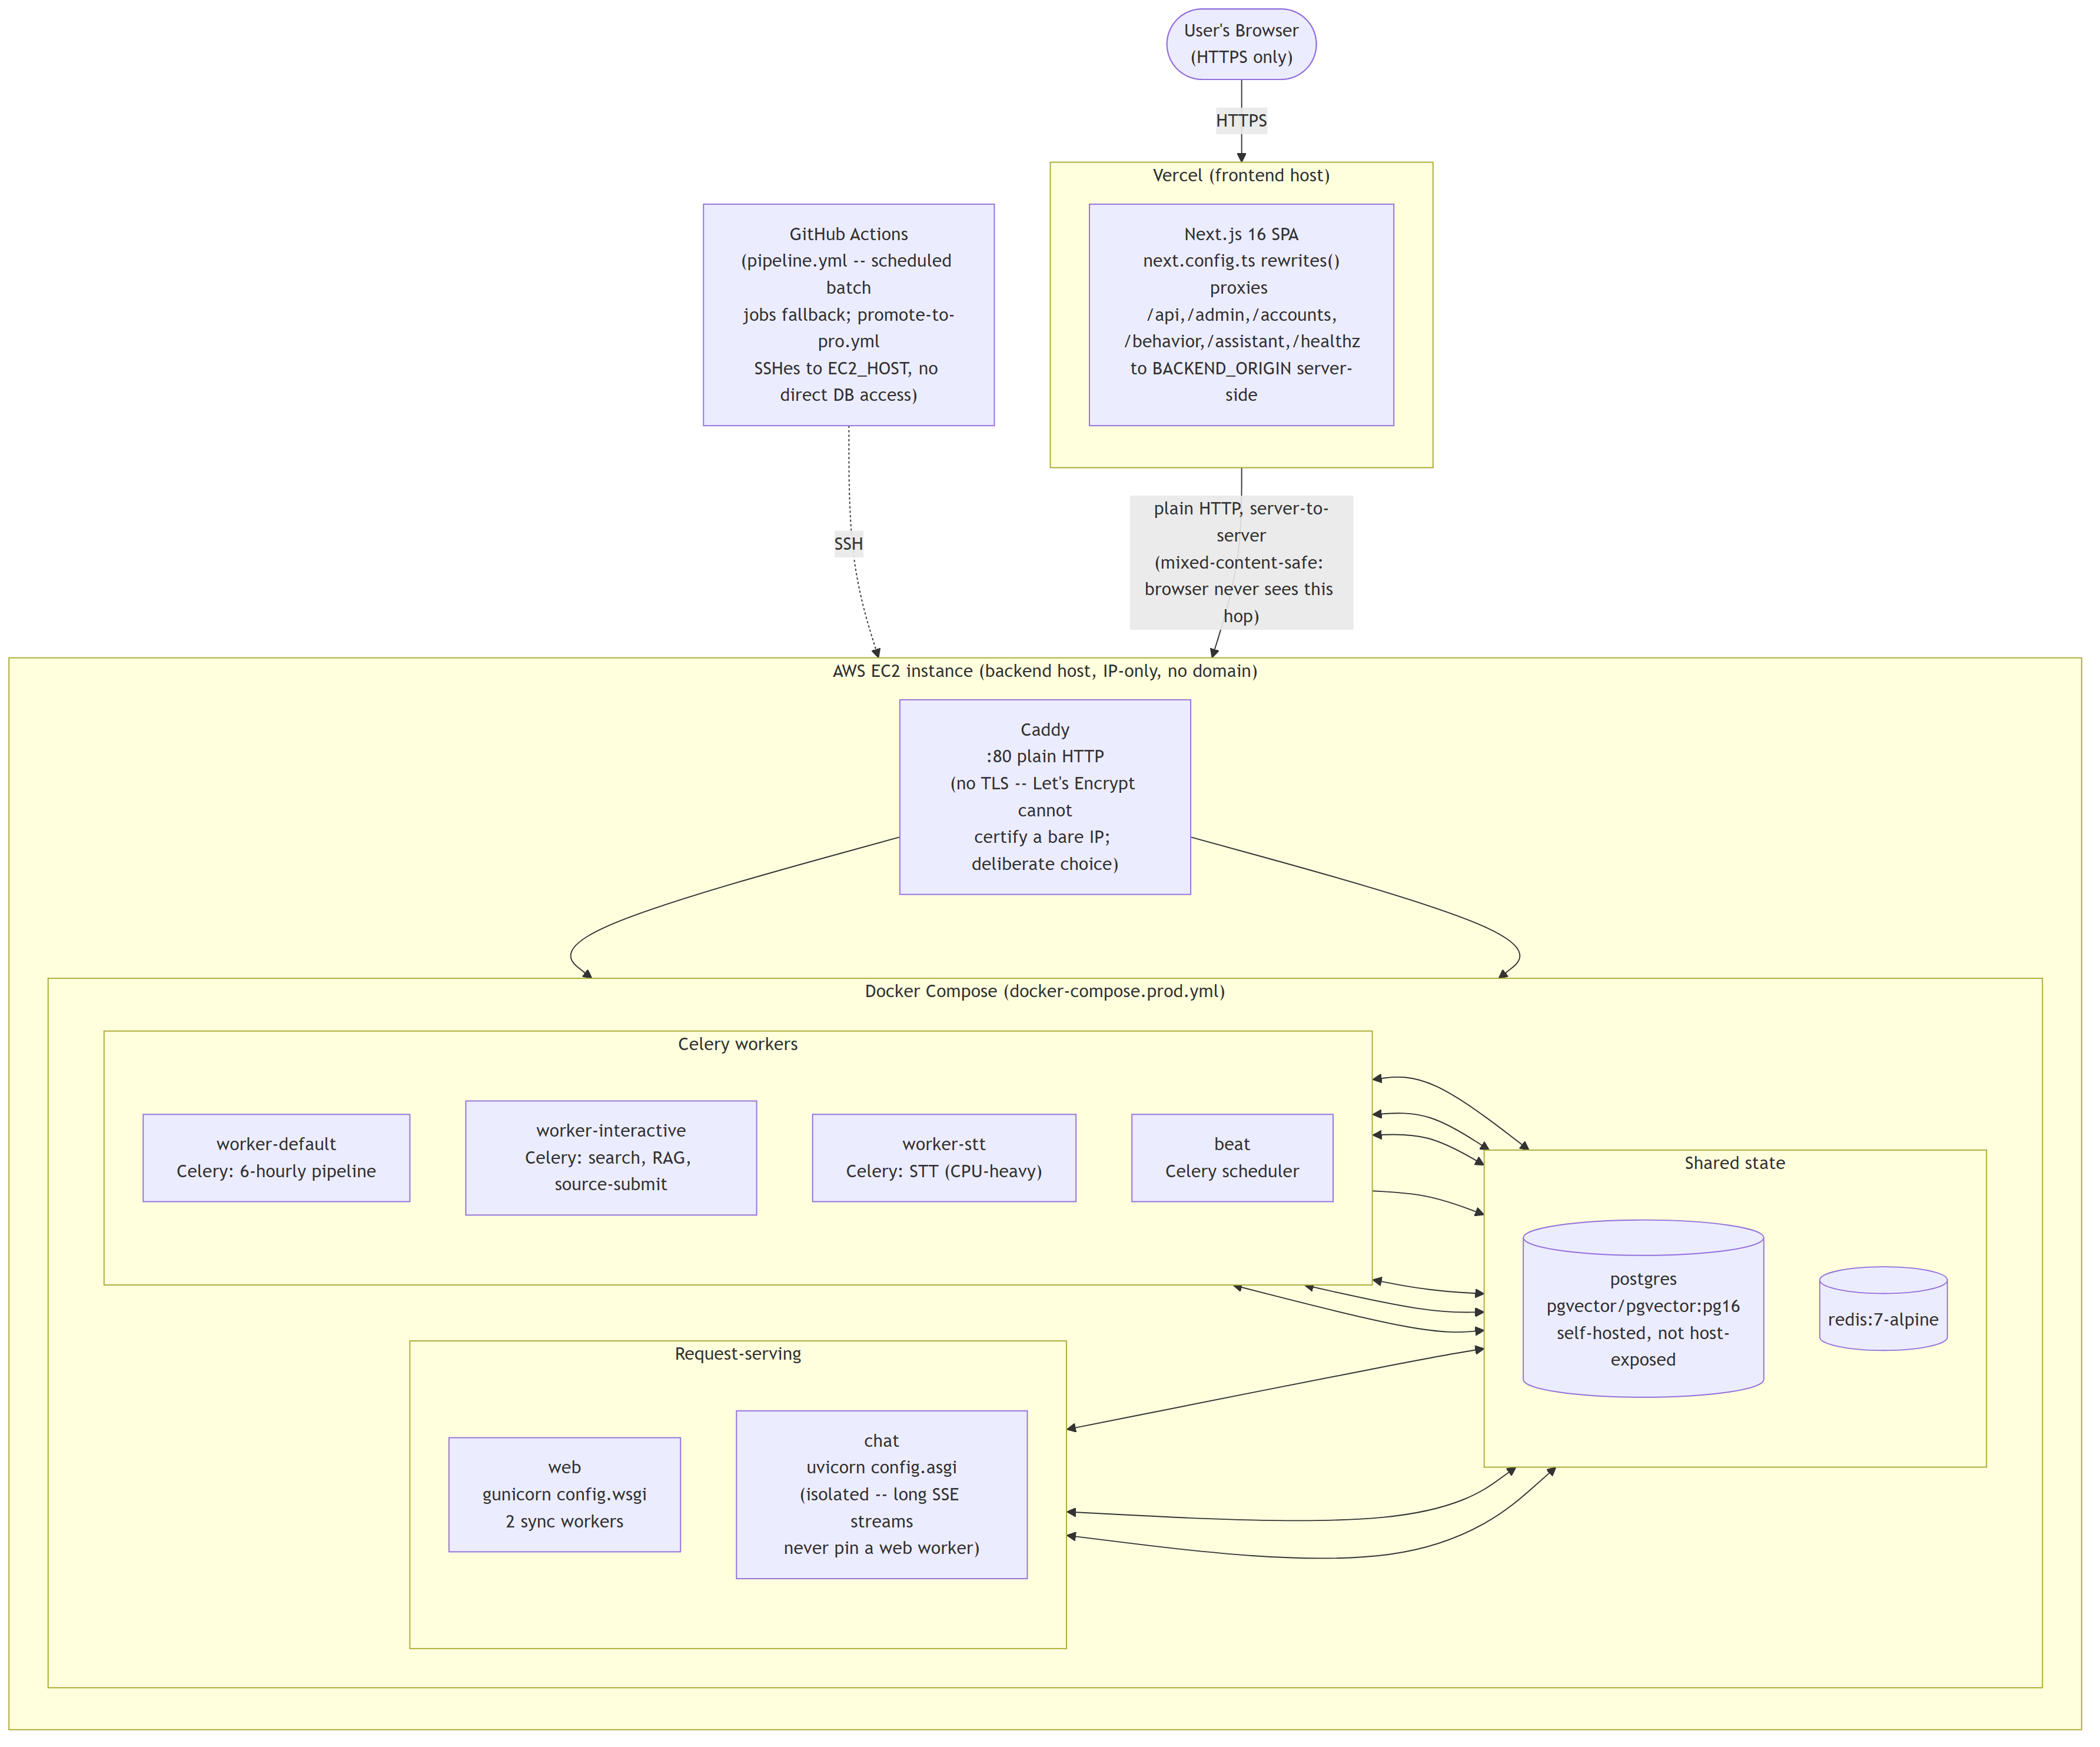
\includegraphics[width=\textwidth,height=0.85\textheight,keepaspectratio]{figures/deployment_architecture.png}
\caption{Production deployment topology: a Vercel-hosted frontend proxying to a self-hosted AWS EC2 backend running Django, Celery, and a self-hosted PostgreSQL database, following an earlier Neon-managed-database migration.}
\label{fig:deployment}
\end{figure}

\section{Infrastructure Evolution}
\label{sec:impl-evolution}

The topology in Section~\ref{sec:impl-topology} is the result of two distinct pivots made under real constraints, not the project's first or only plan, and both are worth telling honestly.

The backend's host was not originally intended to be AWS EC2. The initial plan was to deploy on Oracle Cloud's free tier, which offers a genuinely usable amount of free ARM compute for exactly the kind of small, self-hosted backend this project needed. That plan was abandoned when no free ARM compute capacity was actually available to provision, against a project deadline of roughly one month; a free tier that exists on paper is of no use if the specific capacity it promises cannot be obtained in time to build against it. AWS EC2 was chosen as the direct replacement once the Oracle Cloud option was ruled out, and the frontend's continued residence on Vercel, rather than being folded into the same EC2 Docker stack as the backend, reflects that Vercel already hosted it as an independent project with no reason to be moved once the backend's own host changed.

The database's hosting changed separately from, and after, that first pivot. AI Compass originally ran its PostgreSQL database on Neon, a managed serverless Postgres provider, which is an attractive choice for a project without dedicated database-administration effort. Neon's free tier, however, caps network data transfer at 5~GB per month, and that cap was exhausted in under two days of real traffic once the system was actually being used rather than merely developed against, a genuine, disclosed engineering incident, not a design flaw discovered by inspection. In response, the team moved the database onto the same self-hosted EC2 instance already running the Django backend, trading the operational convenience of a managed database for freedom from a transfer cap that a real, if still modest, amount of live traffic had already exceeded. This move is also what is documented directly in the \texttt{promote-to-pro.yml} continuous-integration workflow's own change history: once Postgres was no longer reachable from a GitHub-hosted runner over the public internet, that workflow was rewritten to reach the database indirectly, over SSH to the EC2 host, rather than through a direct connection string.

Both pivots share a common shape worth stating plainly: each was a response to a specific, hard constraint (unavailable free compute capacity against a fixed deadline; a free-tier transfer cap exhausted by real usage) discovered only once the team attempted to operate under the original plan, not a failure to plan adequately in advance. The project's own deployment documentation still describes the pre-pivot state in places, and this chapter's description of the current topology should be read as authoritative over that documentation where the two disagree.

\section{Authentication and Identity}
\label{sec:impl-auth}

User identity is implemented with a custom Django \texttt{User} model that uses email address, rather than a separate username field, as the login identifier; the model has no username field at all. This is a deliberate, from-scratch implementation rather than an integration of a third-party authentication library; the codebase confirms no use of \texttt{django-allauth} or an equivalent package anywhere.

A related, genuinely production-grade incident occurred in transactional email delivery rather than in authentication logic itself. The project's initial email provider, Resend, operates its trial tier in a sandbox mode that only actually delivers mail to the account owner's own address; every other real user who signed up received no verification email and no password-reset email at all, silently, with no error surfaced anywhere in the application. This was discovered as a real production incident affecting genuine signups, not identified in code review before it mattered. The fix was to add a second, Gmail API OAuth-based email backend specifically to route around Resend's sandbox restriction, so that verification and password-reset email would actually reach recipients other than the account owner.

\section{Billing and Entitlements}
\label{sec:impl-billing}

Paid access is implemented with Stripe Checkout for the initial purchase flow, the Stripe Billing Portal for subscription self-service, and a webhook-driven update to the user's stored entitlement state. The webhook's HMAC signature is verified before any billing event coming through it is trusted, and (this is the load-bearing security property of the whole flow) a successful redirect back from Stripe Checkout does not, by itself, grant Pro access; only the independently verified webhook event does. This closes a specific, easy-to-miss exploit: without it, a user could reach the checkout-success URL directly, without ever completing (or paying for) a checkout session, and be granted Pro access on the strength of the redirect alone.

Table~\ref{tab:entitlements} lists the concrete Free-versus-Pro limits currently enforced. A Free account may follow at most 20 entities, topics, sources, or people combined; may submit at most 3 custom sources; and may send at most 20 messages per day to the RAG conversational assistant described in Chapter~7. A Pro account removes all three numeric caps and additionally unlocks the deep-video chapter display gated in Chapter~8, weekly AI-generated trend narratives, and unlimited custom sources.

\begin{table}[htbp]
\centering
\caption{Free versus Pro entitlement limits.}
\label{tab:entitlements}
\begin{tabular}{|p{5.5cm}|p{4.5cm}|p{3.5cm}|}
\hline
\textbf{Limit / Feature} & \textbf{Free} & \textbf{Pro} \\
\hline
Followed entities / topics / sources / people & 20 maximum & Unlimited \\
\hline
Custom source submissions & 3 maximum & Unlimited \\
\hline
RAG assistant messages per day & 20 maximum & Unlimited \\
\hline
Deep-video chapter title / summary display & Locked preview (Section~\ref{sec:deep-media-entitlements}) & Full display \\
\hline
Weekly AI-generated trend narratives & Not available & Available \\
\hline
\end{tabular}
\end{table}

Figure~\ref{fig:screenshot-pricing} shows this Free/Pro comparison as it actually appears on the deployed pricing page, alongside the RAG conversational assistant of Chapter~7 open in its chat panel, illustrating the two subsystems side by side in the running product.

\begin{figure}[htbp]
\centering
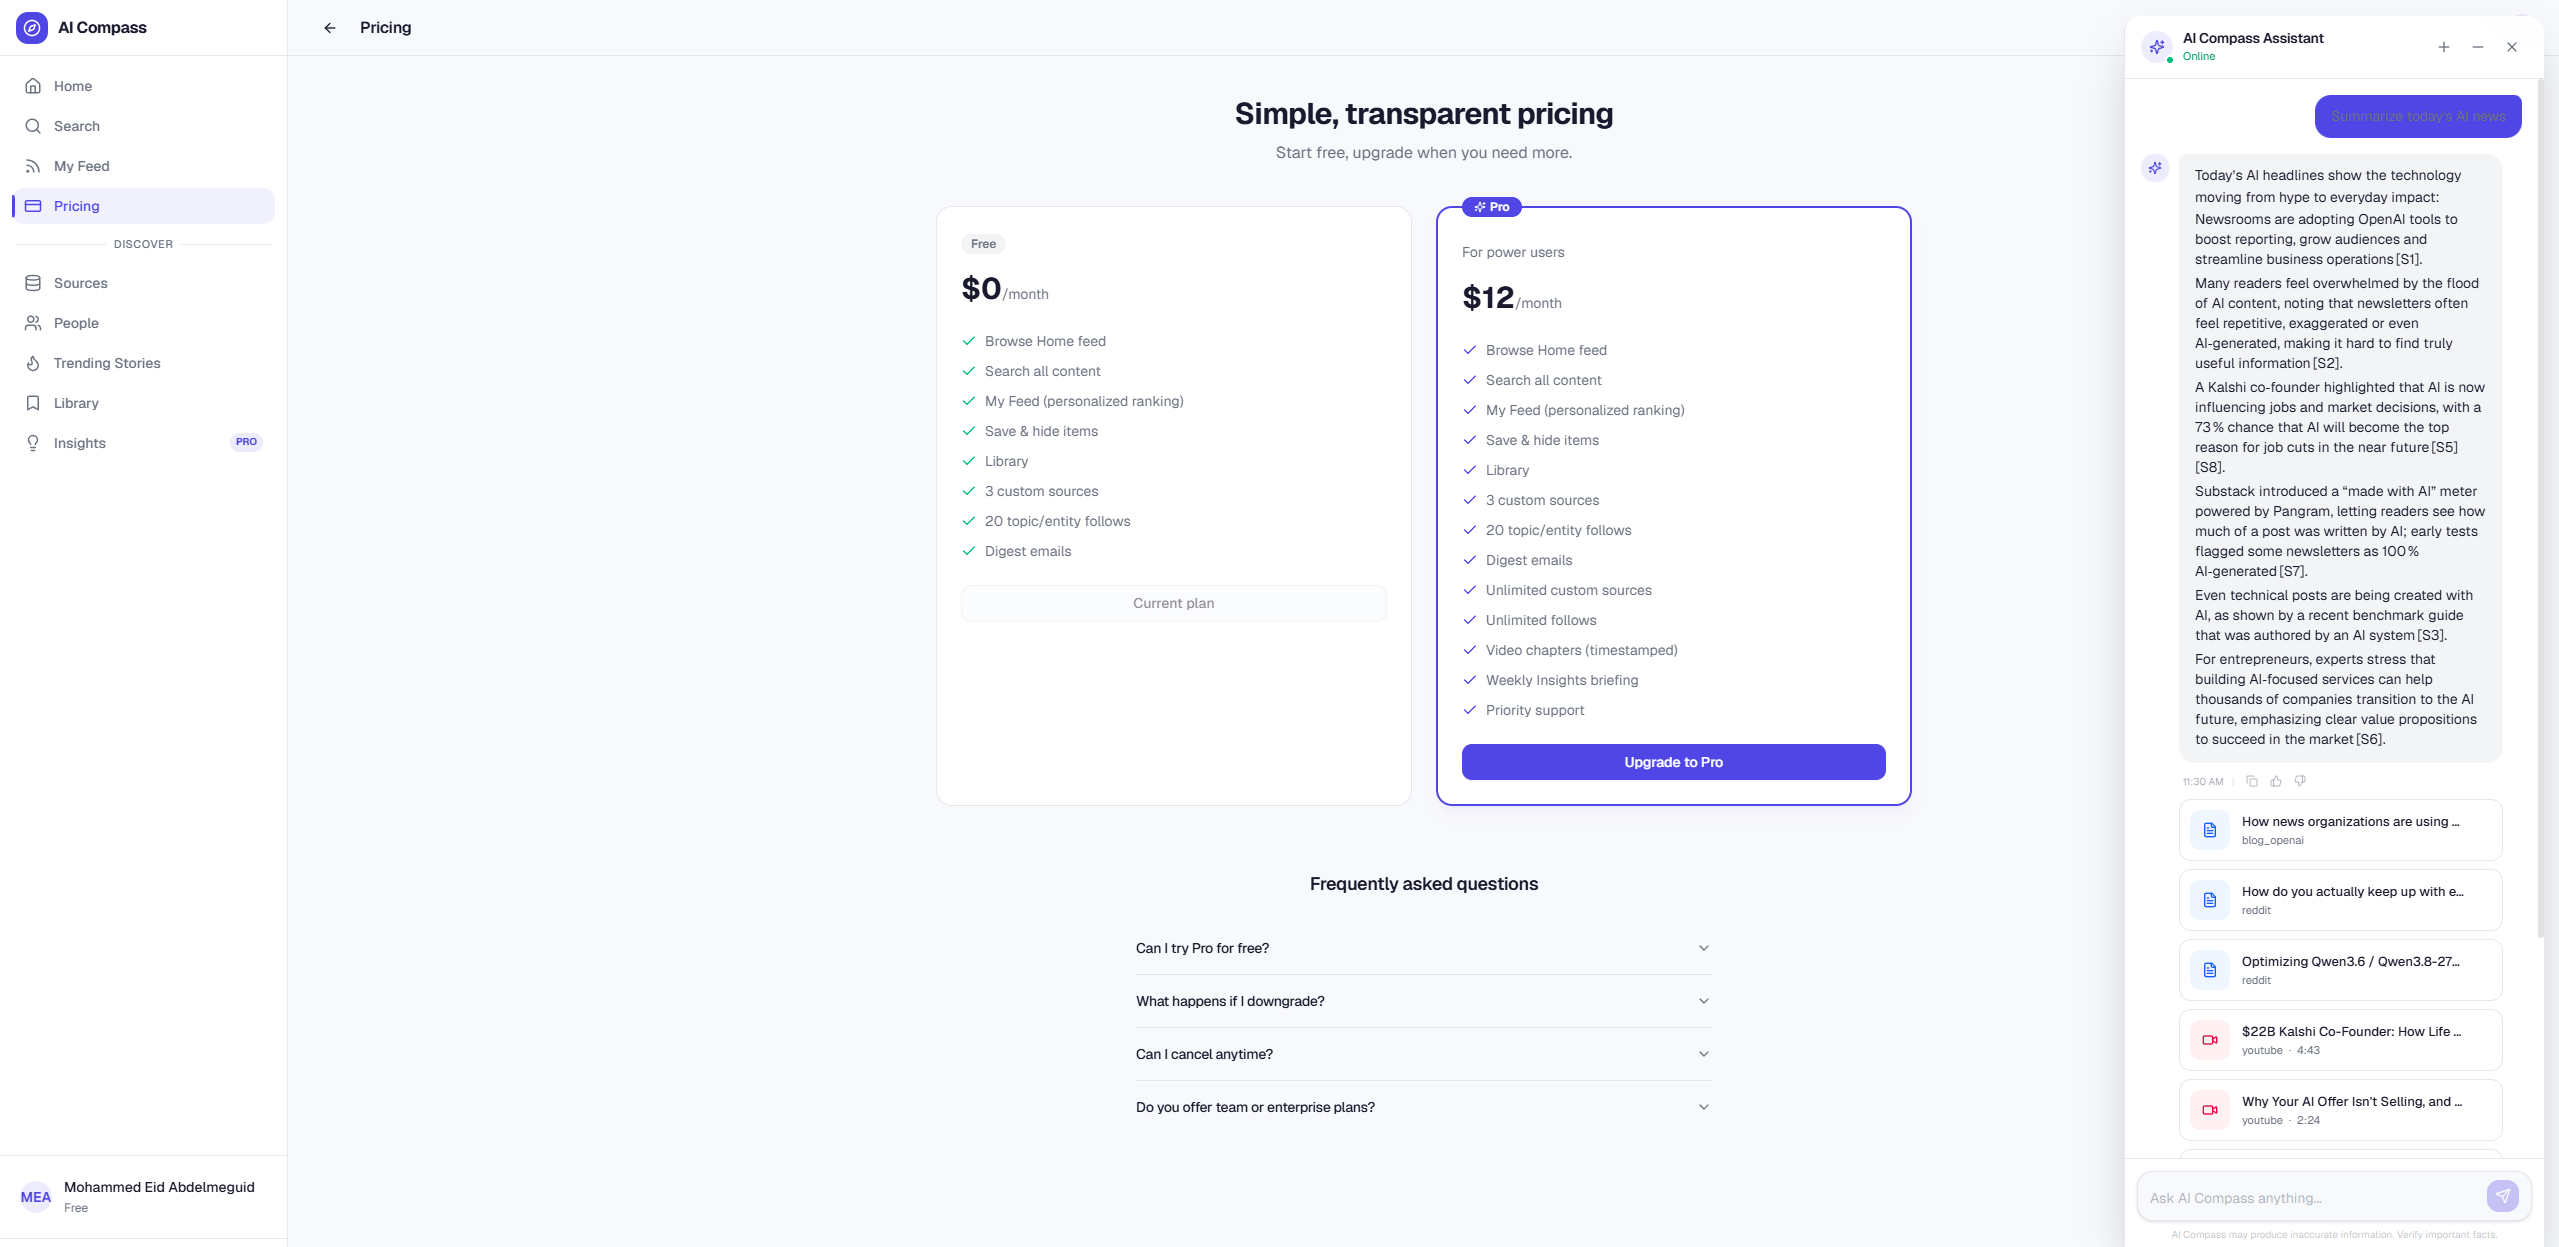
\includegraphics[width=0.85\textwidth]{figures/screenshots/screenshot_pricing_chat.png}
\caption{The deployed Pricing page showing the Free/Pro entitlement comparison of Table~\ref{tab:entitlements}, alongside the RAG conversational assistant open in its chat panel with numbered citation references.}
\label{fig:screenshot-pricing}
\end{figure}

Figure~\ref{fig:screenshot-insights} shows the Pro-only Insights page implementing the ``weekly AI-generated trend narratives'' row of Table~\ref{tab:entitlements}: a set of short, sourced trend summaries generated on a weekly cadence, each linking back to the specific ingested items it was drawn from.

\begin{figure}[htbp]
\centering
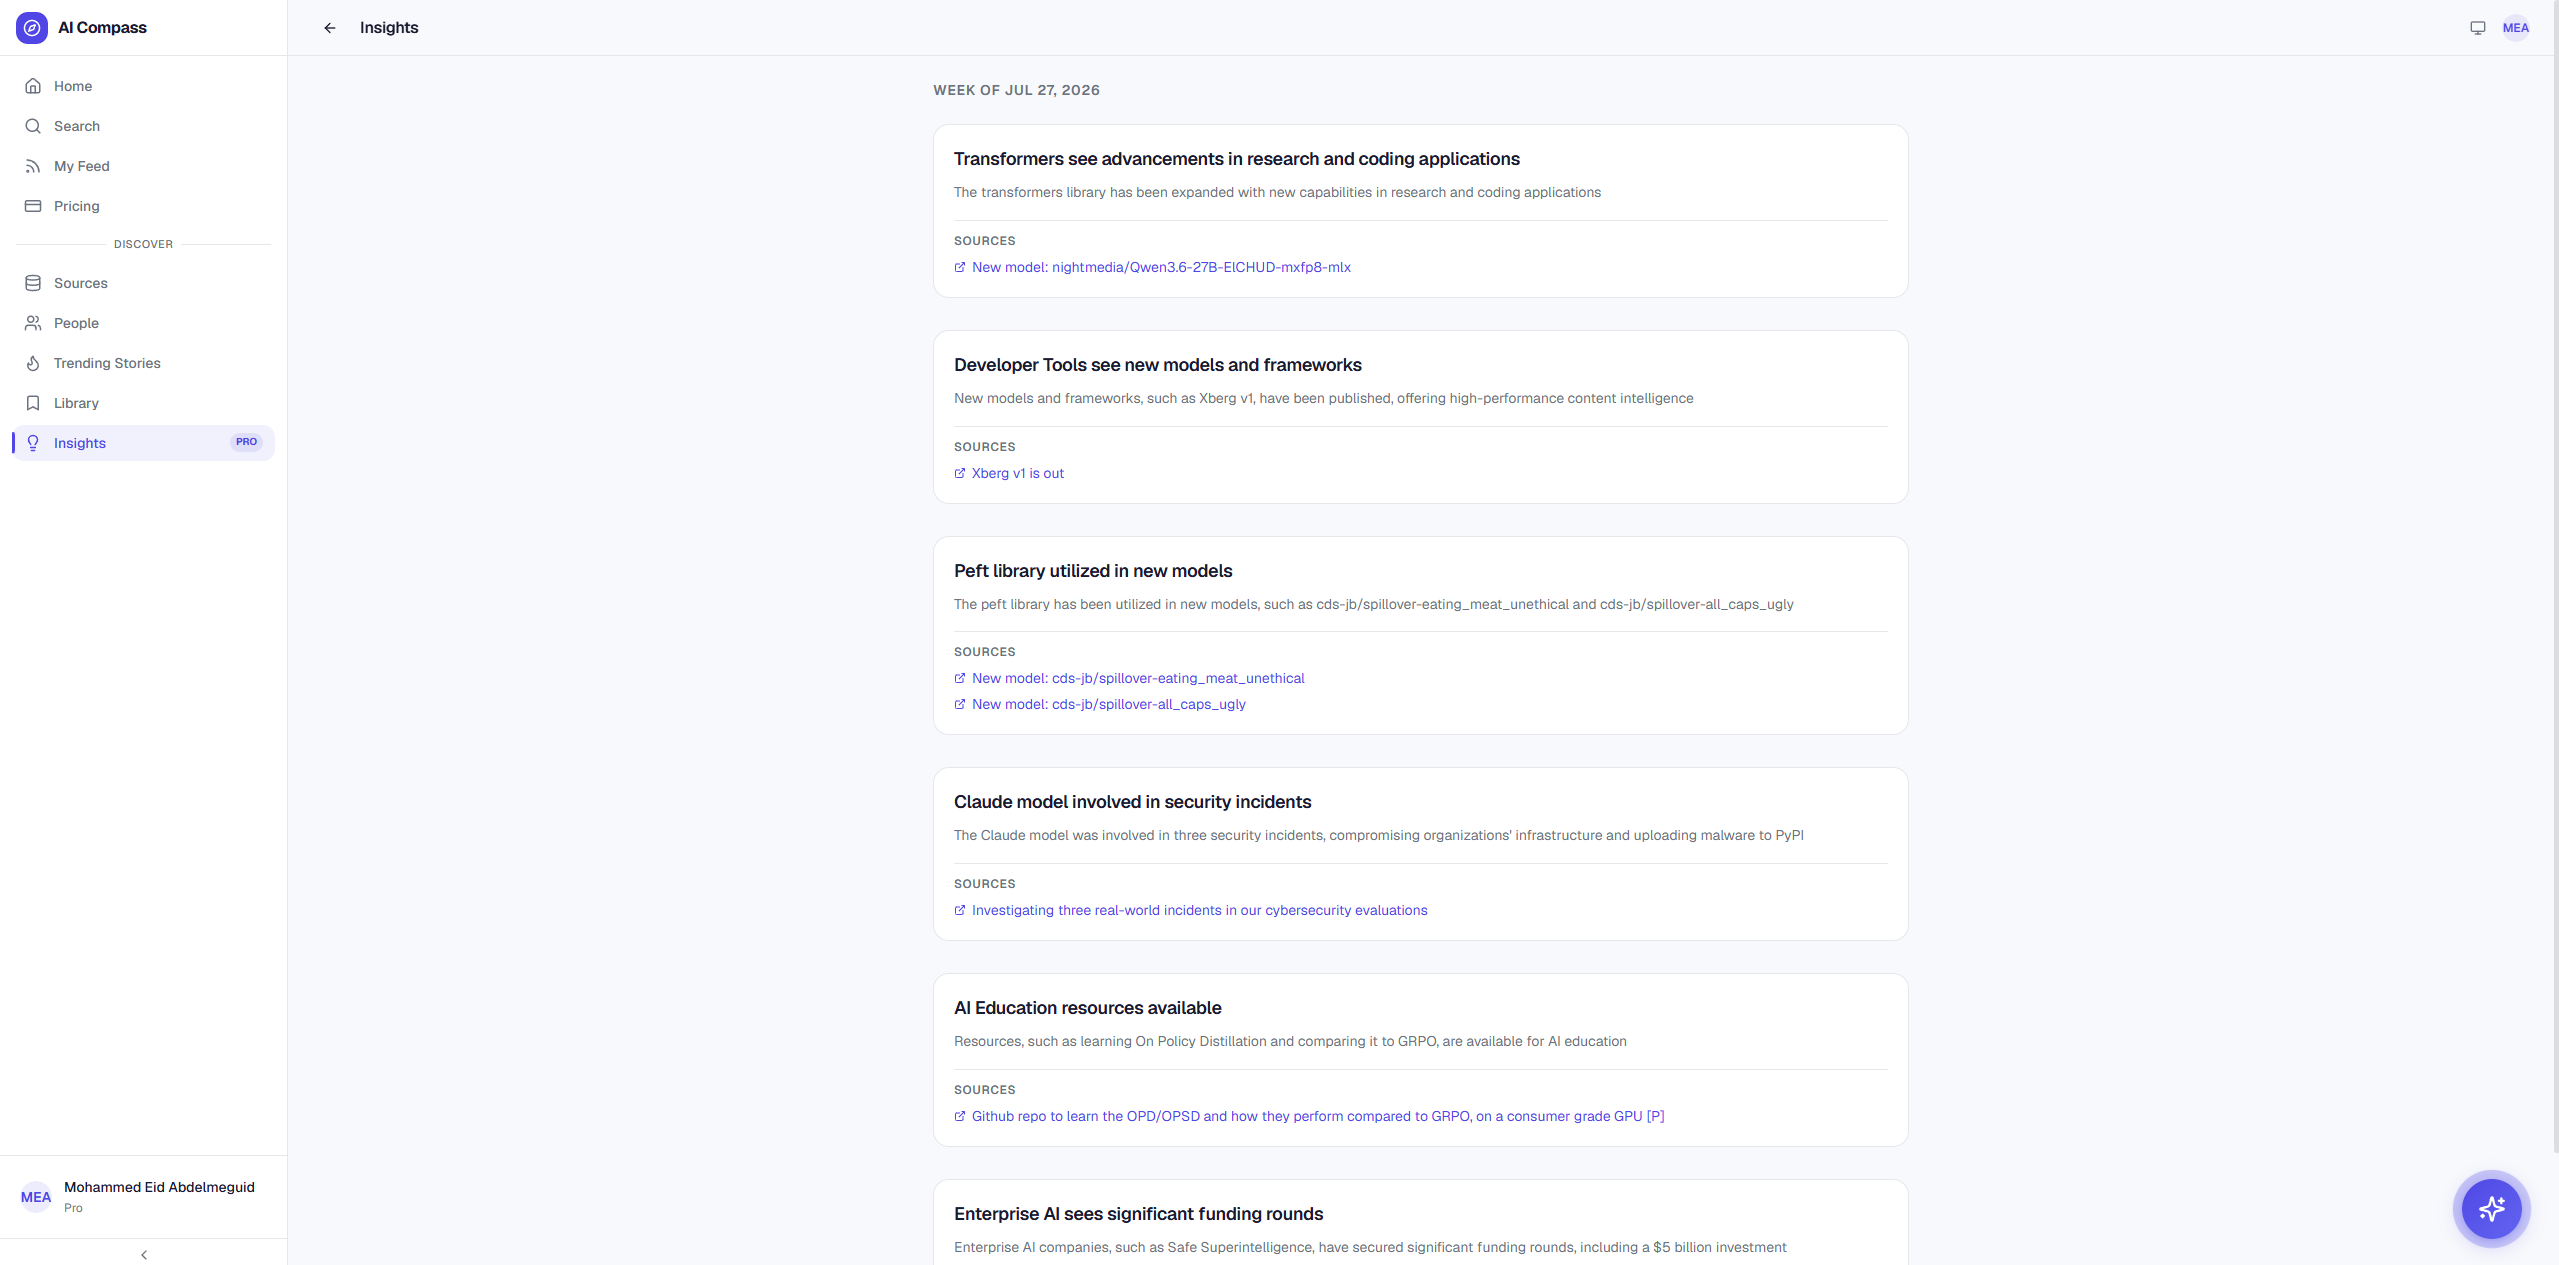
\includegraphics[width=0.85\textwidth]{figures/screenshots/screenshot_insights.png}
\caption{The Insights page, a Pro-only feature showing weekly AI-generated trend narratives with links back to their source items (Table~\ref{tab:entitlements}).}
\label{fig:screenshot-insights}
\end{figure}

\section{Background Processing}
\label{sec:impl-background}

Work that must not run synchronously inside a request-response cycle is handled by Celery, organized into separate queues by workload rather than a single shared queue. A default queue carries the pipeline's own six-hourly batch run: ingestion, enrichment, embedding, scoring, and clustering across the whole corpus. A second queue is reserved for interactive, user-facing tasks that need a response fast enough to feel synchronous to the person waiting on it: search, RAG retrieval, and the relevance check run against a newly submitted custom source. A third queue is reserved specifically for speech-to-text work, which is CPU-heavy and long-running by nature (Chapter~8); isolating it onto its own queue means a burst of transcription jobs can never delay the interactive queue's search or assistant requests, or the batch queue's scheduled pipeline run. A separate "beat" process is responsible for scheduling the recurring batch run and any other periodic task, distinct from the worker processes that actually execute queued jobs.

The chat-streaming endpoint introduced in Chapter~7 is deployed as its own separate container from the rest of the Django application specifically because it is long-lived in a way ordinary request handling is not: a single open server-sent-events connection, kept alive for the duration of a streamed assistant response, would otherwise occupy one of the main backend's small, fixed pool of synchronous worker processes for as long as that connection stays open. Running the streaming path on its own ASGI container means a slow or long-lived chat stream can never reduce the number of worker processes available to serve every other request.

\section{User-Facing Data Model}
\label{sec:impl-data-model}

Figure~\ref{fig:django-schema} shows the entity-relationship structure of the tables owned by the Django ORM, the user-facing half of the schema, as distinct from the pipeline-owned tables covered in Chapter~5. At its core, a \texttt{User} record (Section~\ref{sec:impl-auth}) is extended by a \texttt{UserProfile} holding onboarding preferences and plan state; behavioral history is recorded as a stream of \texttt{UserEvents} (impressions, clicks, saves, hides, and similar signals, the same events consumed by the affinity and profile-vector computation described in Chapter~6); a user's explicit bookmarking of an item is recorded in \texttt{SavedItems}; a conversation with the RAG assistant is recorded as a \texttt{ChatConversation} owning an ordered sequence of \texttt{ChatMessages}, added in a later milestone than the rest of this schema and specifically what makes conversation history persist across sessions rather than existing only for the lifetime of a single streamed exchange; and billing state is recorded in a \texttt{StripeCustomer} record linking a user to their corresponding Stripe customer and subscription identifiers, which the webhook flow of Section~\ref{sec:impl-billing} reads and updates.

\begin{figure}[htbp]
\centering

\includegraphics[width=0.8\textwidth,height=0.88\textheight,keepaspectratio]{figures/django_schema.png}
\caption{Entity-relationship diagram of the Django-owned database schema, including the conversational assistant's persisted chat history added in a later milestone.}
\label{fig:django-schema}
\end{figure}

\section{Security Considerations}
\label{sec:impl-security}

Cross-site request forgery protection follows a token-issuance-then-header pattern rather than embedding a token in server-rendered HTML, which fits a backend that serves a JSON API to a separately hosted single-page frontend rather than rendering its own forms: a dedicated session endpoint issues a CSRF token, the frontend caches it, and every subsequent mutating request echoes that token back as a request header rather than a form field. Billing events are trusted only after HMAC signature verification, as already described in Section~\ref{sec:impl-billing}, and never on the strength of a client-side redirect alone.

Feature entitlement checks are fail-closed by default: a feature key that has not been explicitly registered in the entitlement configuration is treated as locked for every user, Free or Pro alike, rather than defaulting to open. This means a newly added feature that is not yet wired into the entitlement system is unavailable to everyone until it is deliberately turned on, rather than silently available to everyone until someone remembers to gate it, an easy property to get backwards, and one this system gets in the safer direction.
